\documentclass{article}
\usepackage[spanish]{babel}   
\usepackage[numbers,sort&compress]{natbib}
\usepackage{float}
\usepackage{listings}
\usepackage{graphicx} 	% Nos permite importar imagenes 
\usepackage{subcaption}
\usepackage[left=3cm,right=3cm,top=3cm,bottom=3cm]{geometry}

%-------------------------- Por si se romple la URL --------------------------
\usepackage[hyphens]{url}
\usepackage[hidelinks]{hyperref}
\hypersetup{breaklinks=true}	
\urlstyle{same}
\usepackage{cite}
%-------------------------- Por si se romple la URL --------------------------

\title{Reporte Tarea 3}
\author{Victor Alejandro Oviedo Martínez}



\begin{document}
\maketitle
\hrule

\section{Introduccón}\label{intro}

Para esta tercer tarea\citep{DRA.P3} se ha estudiado el tema Teoría de colas, el cual es el estudio de las matemáticas que estudia las lineas de espera en un sistema. Para un mejor entendimiento del tema, se ha propuesto una forma de estudio, en donde se toma como experimento saber si un número es, o no un número primos. Como marco de referencia para la obtención de números primos, tenemos que los números primos solo son divisibles entre uno, y sí mismo. Por lo tanto, detener más de un divisor tendremos que el evaluando no seria número primo.  De esta forma se entiende que para saber si un número es primo, se tendrían que evaluar todos los números hasta  \texttt{(n-1)} y determinar si alguno de estos es divisor, por lo tanto, mientras mayor sea el número mayor será el tiempo que tardaremos en saber si es primo.  Una vez entendido el concepto de número primo podremos avanzar ha entender el multiprocesamiento. En la actualidad existen microprocesadores los cuales tienen más de un núcleo,  de tener mas de un núcleos podremos realizar múltiples tareas al mismo tiempo a diferencia de tener solo uno. Por lo tanto, es de suma importancia entender la forma en la que es suministrada la información a estos núcleos para obtener mejor rendimiento en tiempo. De tal forma que no sirve de mucho tener una gran cantidad de núcleos, si no se sabe suministrar la información, ``With great power, comes great responsibility''.- Uncle Ben. Ahora, realizando una simulación de lo ya explicado, podremos ver las diferencias en el tiempo dependiendo  de la distribución de  información.   \\

%jejajo jejo por \citep{DRA.P3}, jaj y luego \citet{DRA.P3}

\section{Desarrollo}

Para esta tercer tarea se ha planteado el siguiente problema: Examina cómo las diferencias en los tiempos de ejecución de los diferentes ordenamientos cambian cuando se varía el número de núcleos asignados al cluster, utilizando como datos de entrada un vector que contiene primos grandes, descargados de https://primes.utm.edu/lists/small/millions/ y no-primos con por lo menos ocho dígitos. Investiga también el efecto de la proporción de primos y no-primos en el vector igual como, opcionalmente, la magnitud de los números incluidos en el vector con pruebas estadísticas adecuadas.\\

Para el desarrollo de esta tarea se a utilizado el código ejemplo proporcionado por la Dra. \citet{DRA.Code} , el cual tiene el propósito de realizar pruebas con multiprocesamiento a un conjunto de datos, los cuales se les da tres diferentes ordenamientos y con estos diferentes ordenamientos, se espera un tiempo de regreso para observar las diferencias del procesamiento en el tiempo. Esté código será  tomando como base y modificando para las características de esta tarea.\\

La edición de este código  empieza importando datos de un archivo con el nombre \texttt{Datos.txt}, el cual contiene 2860 número primos con 8 dígitos. Estos números quedaran guardados en la variable \texttt{datos}.\\

\begin{lstlisting}[language=Python]
with open('Datos.txt', 'r') as input:
        linea = input.readline()

    datos = [int(valor) for valor in linea.split(',')]
    num_datos = len(datos)
\end{lstlisting}

Una vez guardados los datos, generamos a partir de los valores de la variable \texttt{datos} números no-primos. Esto es posible ya que al tener todos los números primos de un rango, se tiene que los valores entre ellos no son números primos. Por lo tanto, se obtienen la mitad de los números de este rango y se guardan en la variable \texttt{datos-faciles}. Dado que el nombre de las variables con guion bajo entra en conflicto con LaTex se han cambiado en este archivó   el guion bajo, por el guion alto solo en el nombre de las variables remarcadas.\\ 

\begin{lstlisting}[language=Python]
for exp in range(int((num_datos + 1)/2)):
        if exp == 0:
            imp = datos[exp]
            imp2 = datos[exp + 1]
            o = exp + 1
        elif exp > 0:
            imp = datos[o + 1]
            imp2 = datos[o + 2]
            o = o + 2
        #print(imp, imp2, exp)
        for cand in range(imp, imp2+1):
            datos_faciles.append(cand)
\end{lstlisting}

Una vez teniendo datos difíciles como lo son la lista de números  primos, y
datos fáciles como los números no-primos, en base a estos se generaron 
3 combinaciones diferentes. Para la primera combinación tenemos la 
suma de \texttt{datos} con  \texttt{datos-dificiles} en ese orden, y se guardo
en la variable \texttt{D-F}. para la segunda combinación se realiza lo 
mismo pero con el orden inverso, esto fue guardado en la variable
\texttt{F-D}. Por ultimo, para la tercer combinación se copian y se  
revuelven los datos de la variable \texttt{D-F}.\\

\begin{lstlisting}[language=Python]
    D_F = datos
    D_F.extend(datos_faciles)
    F_D = D_F[::-1]
    Aleatorio = D_F.copy()
    shuffle(Aleatorio)
\end{lstlisting}

Una vez teniendo las tres diferentes combinaciones de datos se puede realizar el experimento. Empezamos  con la creación de un ciclo \texttt{for}, el cual tendrá el objetivo de repetir un proceso la cantidad de núcleos que tenga nuestra pc. Dentro de este \texttt{for} encontraremos la creación de un cluster de multiprocessing, con el fin de dependiendo del valore que tenga la variable \texttt{core} el multiprocessing procese con este número de procesadores. Dentro del cluster, tenemos otro ciclo \texttt{for} el cual repetirá el proceso dentro de el, el número de iteraciones que contenga la variable \texttt{replicas}. Dentro de \texttt{replicas} tendremos el proceso para determinar si son primos los datos de las 3 combinaciones ya mencionadas. \\

\begin{lstlisting}[language=Python]
for core in NUCLEOS:
        with multiprocessing.Pool(core) as pool:
            for r in range(replicas):
                t = time()
                pool.map(primo, D_F)
                tiempos["ot"].append(time() - t)
                t = time()
                pool.map(primo, F_D)
                tiempos["it"].append(time() - t)
                t = time()
                pool.map(primo, Aleatorio)
                tiempos["at"].append(time() - t)
 \end{lstlisting}

Dentro todavía del ciclo \texttt{for} que controla núcleos, se encuentra un nuevo ciclo \texttt{for} pero esta vez para obtener los datos obtenidos por el procesamiento de la información.\\

\begin{lstlisting}[language=Python]
for tipo in tiempos:
            print("")
            print(describe(tiempos[tipo]))
            print("")
            if core == 1:
                grafica1.append(tiempos[tipo])
            elif core == 2:
                grafica2.append(tiempos[tipo])
            elif core == 3:
                grafica3.append(tiempos[tipo])
            elif core == 4:
                grafica4.append(tiempos[tipo])

        pg1.append(np.mean(tiempos["ot"]))
        pg2.append(np.mean(tiempos["it"]))
        pg3.append(np.mean(tiempos["at"]))

        tiempos = {"ot": [], "it": [], "at": []}
 \end{lstlisting}
 
  De tal forma que lo último en este código será la impresión de las figuras.
  Para el desarrollo de esta tarea se utilizaron las siguientes paginas: \citep{DRA.Medicion}, \citep{DRA.Computo}, \citep{DRA.usobasico}.\\ 

\section{Conclusión}

Como conclusión a esta tercer tarea, se ha simulado el programa con las características pedidas. A continuación se podrá observar los resultados. En esta se tiene parte de la respuesta que el programa genera a lo largo de la simulación. Se le han quitado los acentos a esta parte por conflictos con LaTex. Los datos completos estarán en el archivo \texttt{Tarea3.txt}  \\


\begin{lstlisting}[language=Python]



Este programa corre en una pc con 4 nucleos, de los cuales 2 son nucleos virtuales.

Para este programa se han importado 2680  numeros primos, desde 67867979 hasta 67916099  lo que conforma la variable datos. De esta variable se han obtenido los intervalos de 
numeros no-primos para generar la variable datos\_faciles.

Dado que para este programa se tienen 2680 numeros primos, y 25406 numeros no-primos. 
Por lo tanto, se tiene  9 \% de numeros primos, y un 90 \% de numeros no-primos.

----------------------- 1 -----------------------

DescribeResult(nobs=10, minmax=(1.9757118225097656, 3.1582839488983154), 
mean=2.143871212005615, variance=0.12849967295345674, skewness=2.6100195577759018, 
kurtosis=4.935838556729028)


DescribeResult(nobs=10, minmax=(1.966399908065796, 2.1410818099975586), 
mean=2.028838062286377, variance=0.003117389772988746, skewness=0.8193194321308167, 
kurtosis=-0.5071153393493808)


DescribeResult(nobs=10, minmax=(1.988929033279419, 2.135000705718994), 
mean=2.0425031185150146, variance=0.0027558670127771417, skewness=0.47033095855467855, 
kurtosis=-1.1438969573407596)

----------------------- 1 -----------------------

                        *
                        *
                        *
                        
----------------------- 4 -----------------------

DescribeResult(nobs=10, minmax=(1.1669790744781494, 2.9534590244293213), 
mean=1.402350091934204, variance=0.3013912959645899, skewness=2.5952686648917624, 
kurtosis=4.886999007584875)


DescribeResult(nobs=10, minmax=(1.2147572040557861, 1.3716938495635986), 
mean=1.2592074155807496, variance=0.003078004845141575, skewness=1.027304362865847, 
kurtosis=-0.4318316719079771)


DescribeResult(nobs=10, minmax=(1.1185519695281982, 1.2376859188079834), 
mean=1.14898362159729, variance=0.0021672141545877825, skewness=1.2104278873436451, 
kurtosis=-0.281142140033805)

----------------------- 4 -----------------------
-------------------- Global ---------------------

[2.143871212005615, 1.2239134311676025, 1.366836380958557, 1.402350091934204]


[2.028838062286377, 1.5140131950378417, 1.40011568069458, 1.2592074155807496]


[2.0425031185150146, 1.1119722366333007, 1.132978343963623, 1.14898362159729]

-------------------- Global ---------------------
 \end{lstlisting}

Como se ha podido observar en el  código anterior, se tiene la respuesta del programa al momento de ser ejecutado. Al principio se tiene información acerca del procesador de la computadora en la que corre el program. Después, nos habla acerca de las características  de los datos importados y generados, así como la proporción entre primos y no-primos.
Es en este momento en el cual empieza a realizar las simulaciones para los diferentes valores de núcleos, una vez finalizada la simulación de un núcleo en particular imprimirá los resultados obtenidos. Por último, genera las gráficas de la Figura \ref{fig:cuadro.1}, y   entrega  la media  de tiempo para las tres diferentes combinaciones en las 4 diferentes cantidades de núcleos, para luego generar la Figura \ref{fig:cuadro.2}.\\

Cómo observación se realizó el monitoreo de actividad al momento de la simulación, estó se podrá observar en la Figura \ref{fig:cuadro.3}. Esto se hizo con la finalidad de entender si se pude utilizar con seguridad el máximo de núcleos, a lo que la respuesta seria no, ya que si se esta realizando mas de un proceso pesado en la pc esta sube su consumo de procesamiento. Por ejemplo, en la Figura \ref{fig:cuadro.3} se puede observar una grafica semi-escalonada, la cual esta conformada por dos colores, el color azul se refiere al consumo de procesamiento por el usuario, mientras el color rojo es el consumo del sistema. Una vez iniciada la simulación se puede observar como el consumo del usuario incremento hasta no más del 30\% del procesamiento total, esto se mantiene hasta que vuelve a subir hasta no más del 50\%  del procesamiento. Con este comportamiento se puede intuir que a cada incremento corresponde al inicio de un nuevo proceso con mas núcleos. Una vez llegado al procesamiento con los cuatro núcleos se tiene que el mismo sistema no entrega el 100\% del procesamiento , sino que limita este a no mas del 80\% de procesamiento. Sin embargo, de ejecutar otros procesos diferentes a \texttt{Python} el sistema utilizara el 20\% restante. \\


\begin{figure}[H]
\begin{center}
	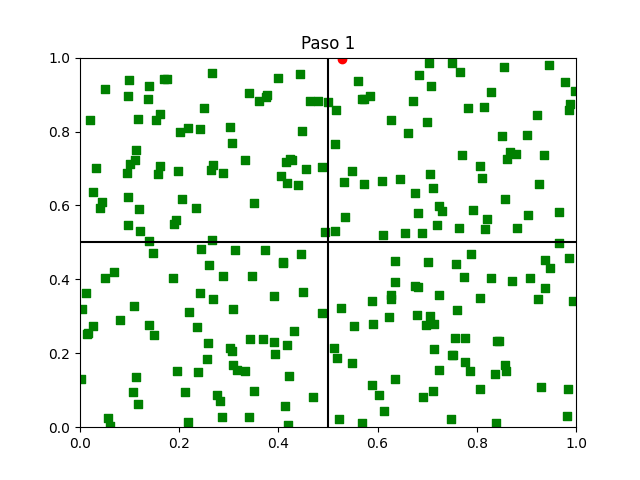
\includegraphics[height=1in]{/Users/victor/Desktop/Figure_3.png}
	\caption{Monitoreo de actividad al momento de ejecución del programa.}
	\label{fig:cuadro.3}
\end{center}
\end{figure}



\begin{figure}[H]
\begin{center}
	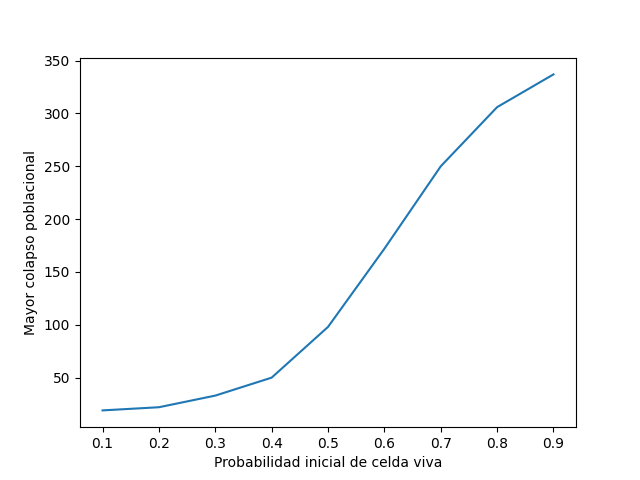
\includegraphics[height=3in]{/Users/victor/Desktop/Figure_1.png}
	\caption{ Resultados de la simulación a 10 repeticiones (tiempo VS combinación).}
	\label{fig:cuadro.1}
\end{center}
\end{figure}

\begin{table}[H]
\centering
\caption{Datos de la simulación a 10 repeticiones (tiempo VS núcleos).}
\label{fig:cuadro1}
\begin{tabular}{|c|c|c|c|}
\hline
Núcleos    &     D\_F    &     F\_D    &     Aleatorio\\
\hline
1& 2.143871212005615 & 2.028838062286377 & 2.0425031185150146 \\
2& 1.2239134311676025&  1.5140131950378417& 1.1119722366333007\\
3& 1.366836380958557&  1.40011568069458 & 1.132978343963623 \\
4& 1.402350091934204& 1.2592074155807496 & 1.14898362159729 \\

\hline
\end{tabular}
\end{table}

\begin{figure}[H]
\begin{center}
	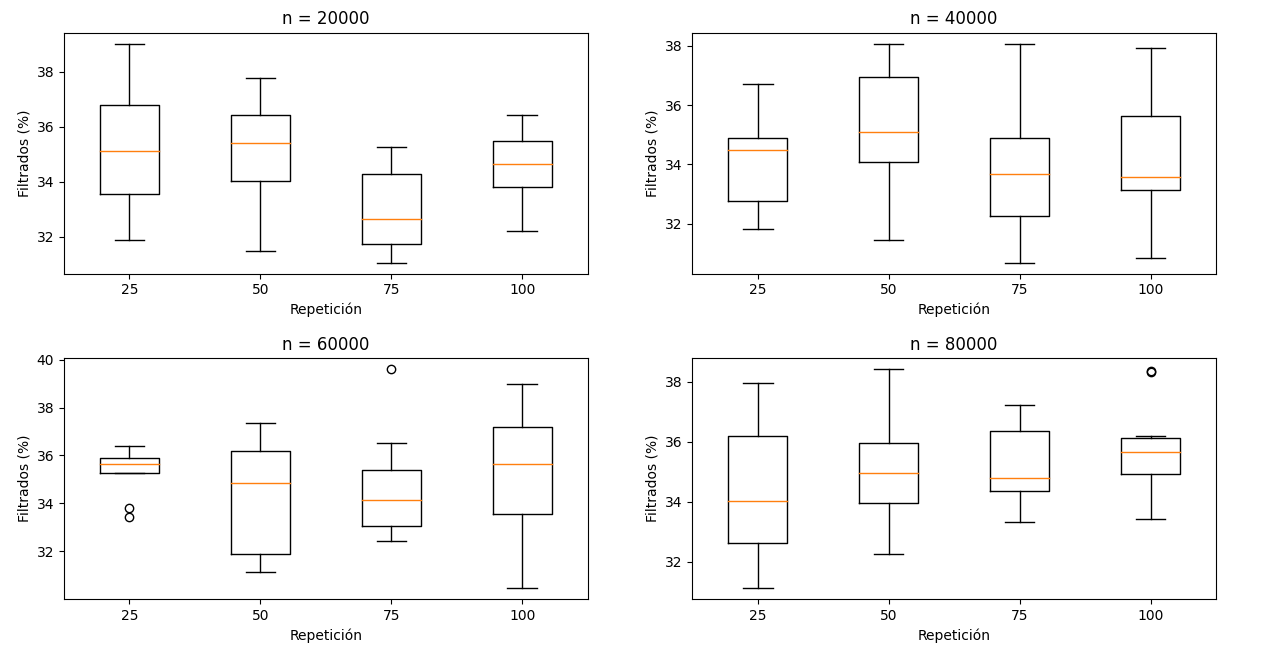
\includegraphics[height=3in]{/Users/victor/Desktop/Figure_2.png}
	\caption{Resultados de la simulación a 10 repeticiones (tiempo VS núcleos).}
	\label{fig:cuadro.2}
\end{center}
\end{figure}









%-------------------------- Por si se romple la URL --------------------------
\Urlmuskip=0mu plus 1mu\relax
%-------------------------- Por si se romple la URL --------------------------
\bibliography{ref.Tarea3.bib}
\bibliographystyle{plainnat}

\end{document}
